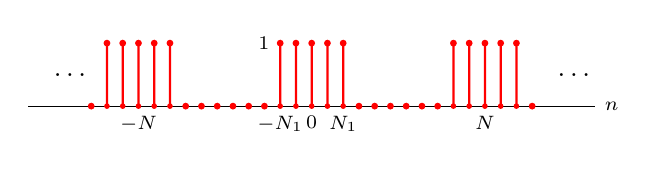
\begin{tikzpicture}[scale=0.8]

	\def\nmin{-13}
	\def\nmax{13}	
	
	\begin{scope}	
		\def\x{{0, 1, 1, 1, 1, 1, 0, 0, 0, 0, 0, 0, 1, 1, 1, 1, 1, 0, 0, 0, 0, 0, 0, 1, 1, 1, 1, 1, 0}}	

		\draw (-4.25, 0) -- (4.75, 0) node[anchor=west] {\scriptsize $n$};
		\foreach \n/\l in {-10/{-N}, -1/{-N_1}, 1/0, 3/{N_1}, 12/{N}}
		{
			\node at (\n/4, 0) [anchor=north] {\scriptsize $\l$};
		}
		\node at (-0.75,1) [anchor=west] {\scriptsize $1$};
		\node at (4,0.5) [anchor=west] {$\dots$};
		\node at (-4,0.5) [anchor=west] {$\dots$};
		
		\foreach \n in {0,1, ..., 28}
		{
			\pgfmathparse{\x[\n]}
			\edef\xn{\pgfmathresult}	
			\ifthenelse{\xn > 0}
			{
				\draw[red, thick, fill=red]  (\n/4 + \nmin/4, 0) -- ++(0, \xn) circle (1pt);% node[anchor=east] {\scriptsize $\xn$};
			}
			{
				\draw[red, fill=red] (\n/4+ \nmin/4,  0) circle (1pt);
			}
		}
	\end{scope}	
\end{tikzpicture}